\documentclass[11pt]{article}
\usepackage[a4paper,margin=1in]{geometry}
\usepackage{amssymb,amsmath,amsthm,mathtools}
\PassOptionsToPackage{hyphens}{url}
\usepackage{hyperref}
\usepackage{enumitem}
\usepackage{microtype}
\usepackage{booktabs}
\usepackage{tabularx}
\newcolumntype{Y}{>{\raggedright\arraybackslash}X}
\usepackage{graphicx}
\usepackage{url}
\usepackage{tikz}
\usetikzlibrary{positioning,arrows.meta}

\title{Strong Normalization for the Safe Fragment of a Minimal Rewrite System:\\
A Triple-Lexicographic Proof and a Conjecture on the Unprovability of Full Termination for Any Relational Operator-Only TRS}
\author{Moses Rahnama\\
\small Mina Analytics}
\date{November 24, 2025}

\newtheorem{theorem}{Theorem}
\newtheorem{lemma}{Lemma}
\newtheorem{definition}{Definition}
\newtheorem{conjecture}{Conjecture}
\newtheorem{corollary}{Corollary}
\theoremstyle{remark}
\newtheorem{remark}{Remark}
\theoremstyle{plain}

\begin{document}
\maketitle

\begin{abstract}
We present a minimal operator-only term rewriting system with seven constructors and eight reduction rules. Our main contribution is a mechanically-verified proof of strong normalization for a guarded fragment using a novel triple-lexicographic measure combining a phase bit, multiset ordering (Dershowitz-Manna), and ordinal ranking. From strong normalization, we derive a certified normalizer with proven totality and soundness. Assuming local confluence (verified through critical pair analysis), Newman's Lemma yields confluence and therefore unique normal forms \emph{for the safe fragment}. We establish impossibility results showing that simpler measures, such as additive counters, polynomial interpretations, and single-bit flags, provably fail for rules with term duplication. The work demonstrates fundamental limitations in termination proving for self-referential systems. We state a conjecture: no \emph{relational} operator-only TRS can have its full-system termination proved by internally definable methods. Here ``relational'' is equivalent to ``capable of ordered computation'': systems with a recursor enabling iteration over successors, comparison, or sequential counting. Such recursors necessarily redistribute step arguments across recursive calls, defeating all additive termination measures. This structural limitation applies to any TRS expressive enough to encode ordered data. All theorems have been formally verified in a proof assistant. The Lean formalization is available at \url{https://github.com/MosesRahnama/OperatorKO7}.
\end{abstract}

\section{Introduction}
\label{sec:intro}
We develop a minimal \emph{operator-only} rewrite calculus (\textbf{KO7}): the object language contains only constructors and operators with rewrite rules; there are no binders, types, external axioms, or semantic predicates. The rules \emph{are} the semantics. Our goals are: (i) a clean, duplication-robust proof of \emph{strong normalization} (SN); (ii) a \emph{certified normalizer} that always returns a normal form; (iii) (optionally) \emph{unique} normal forms via Newman's Lemma under a local-confluence assumption; and (iv) a conjecture that no operator-only TRS capable of ordered computation can have its full-system termination proved by internally definable methods.

\emph{Scope.} All formal results are established for a \emph{guarded safe subrelation}. We do \emph{not} claim a single global measure for the full unguarded relation. Moreover, we exhibit a precise negative: at the root peak $\mathrm{eqW}\,a\,a$ with $\kappa^{M}(a)=0$, local join \emph{fails} in the full relation. Therefore the full relation is not locally confluent at that peak, hence not confluent. The designed remedy is to work in the safe fragment with guarded/context joiners (\S\ref{sec:newman}).

A second conceptual goal is to situate KO7 against results about \emph{fixed-target} reachability in terminating TRSs. If we define an internal provability predicate by ``$t$ reduces to $\top$'', then under SN the set $\{t \mid t \Rightarrow^{\ast} \top\}$ is decidable by normalization/backtracking. With confluence, decision reduces to normal-form equality. This explains why single-level G\"odel encodings cannot coexist with globally terminating proof search; the right move is \emph{stratification}.

\paragraph{Contributions.} (1) A duplication-robust SN proof for KO7 using a triple-lex measure with a multiset (DM) component and an MPO-style head precedence; (2) a total, proved-correct normalizer; (3) a guarded Newman module for the safe relation that yields confluence (hence unique normal forms) from SN + local confluence; (4) a decidability result for reachability under SN; (5) a catalog of impossibility results for additive and polynomial measures under duplication; (6) a formal verification of all results; (7) a conjecture on undecidable termination for operator-only systems within a fixed base theory.

\paragraph{Highlights (formalization summary).}
\begin{itemize}[leftmargin=1.3em]
  \item \textbf{SN (SafeStep) via triple lex}: Formally proven using a lexicographic measure combining a $\delta$-phase bit, a Dershowitz-Manna multiset rank, and an ordinal.
  \item \textbf{Certified normalizer}: A total and sound normalization function is defined by well-founded recursion.
  \item \textbf{Newman (SafeStep)}: Confluence is established via Newman's Lemma using a verified local confluence property for the safe fragment.
  \item \textbf{Full Step caveat}: We exhibit a specific peak ($\mathrm{eqW}\,a\,a$ with $\kappa^M(a)=0$) where local join fails, justifying the restriction to the safe subrelation.
  \item \textbf{Impossibility results}: The failure of simpler additive and polynomial measures is formally witnessed by counterexamples.
\end{itemize}

\section{Background: TRSs, SN, reachability, and Newman}
\label{sec:background}
We assume standard abstract reduction and term rewriting notions \cite{BaaderNipkow98,Terese03}. A term is in \emph{normal form} if no rule applies. A TRS is \emph{strongly normalizing} (SN) if there are no infinite reductions. A relation is \emph{confluent} if for any $t \Rightarrow^{\ast} u$ and $t \Rightarrow^{\ast} v$ there exists $w$ with $u \Rightarrow^{\ast} w$ and $v \Rightarrow^{\ast} w$. \emph{Local confluence} requires this only for single-step forks. \emph{Newman's Lemma} asserts SN + local confluence $\Rightarrow$ confluence \cite{Newman42}, yielding unique normal forms.

Fixed-target (``small-term'') reachability in terminating TRSs has well-charted complexity: NP-complete for length-reducing systems (dropping to P under confluence), NExpTime/N2ExpTime for (linear) polynomial interpretations, and PSPACE for KBO-terminating TRSs \cite{BaaderGiesl24}. Modularity holds in certain linear, non-collapsing combinations \cite{CaronCoquide94}, while even \emph{flat} non-linear systems exhibit undecidable reachability and confluence \cite{Mitsuhashi06}. Termination under duplication typically requires orders beyond plain sizes; a naive size can increase under duplicating rules. The cure is a \emph{multiset} extension of a base order \cite{DershowitzManna79} or (recursive) path orders \cite{Dershowitz87}.

\section{The KO7 calculus}
\label{sec:ko7}
KO7 is a finite TRS over a small signature (7 constructors) with 8 rules (including the equality-witness operator \texttt{eqW}). For concreteness we list the kernel rule shapes below.

\begin{table}[h]
  \centering
  \begin{tabular}{@{}llcll@{}}
    \toprule
    Rule & Head & Arity & Shape & Dup? \\
    \midrule
    \texttt{R\_merge\_void\_left} & merge & 2 & $\mathrm{merge}\;\mathrm{void}\;t \to t$ & No \\
    \texttt{R\_merge\_void\_right} & merge & 2 & $\mathrm{merge}\;t\;\mathrm{void} \to t$ & No \\
    \texttt{R\_merge\_cancel} & merge & 2 & $\mathrm{merge}\;t\;t \to t$ & No \\
    \texttt{R\_rec\_zero} & rec$\Delta$ & 3 & $\mathrm{rec}\,\Delta\,b\,s\,\mathrm{void} \to b$ & No \\
    \texttt{R\_rec\_succ} & rec$\Delta$ & 3 & $\mathrm{rec}\,\Delta\,b\,s\,(\mathrm{delta}\,n) \to \mathrm{app}\,s\,(\mathrm{rec}\,\Delta\,b\,s\,n)$ & No$^*$ \\
    \texttt{R\_int\_delta} & integrate & 1 & $\mathrm{integrate}\,(\mathrm{delta}\,t) \to \mathrm{void}$ & No \\
    \texttt{R\_eq\_refl} & eqW & 2 & $\mathrm{eqW}\;a\;a \to \mathrm{void}$ & No \\
    \texttt{R\_eq\_diff} & eqW & 2 & $\mathrm{eqW}\;a\;b \to \mathrm{integrate}\,(\mathrm{merge}\,a\,b)$ & No \\
    \bottomrule
  \end{tabular}
  \caption{KO7's 8 kernel rules. In the full kernel relation, \texttt{R\_eq\_refl} and \texttt{R\_eq\_diff} overlap at \texttt{eqW a a}. The certified safe fragment guards \texttt{R\_eq\_diff} by $a \neq b$. \texttt{R\_merge\_cancel} is collapsing. $^*$\texttt{R\_rec\_succ} redistributes $s$ to two RHS positions.}
\end{table}

\paragraph{Kernel signature (7 constructors).}
Terms are generated by the constructors:
\[
t ::= \mathrm{void}
\mid \delta\,t
\mid \mathrm{integrate}\,t
\mid \mathrm{merge}\,t\,t
\mid \mathrm{app}\,t\,t
\mid \mathrm{rec}\,\Delta\,t\,t\,t
\mid \mathrm{eqW}\,t\,t.
\]
The full kernel relation \texttt{Step} is generated by the 8 rules in Table~1, while the certified artifact is proved for a guarded subrelation \texttt{SafeStep}.

\paragraph{Tiny example (trace consequences).} Using the verified normalizer, we observe:
\begin{itemize}[leftmargin=1.4em]
  \item Integrate/delta: $\mathrm{integrate}(\delta\,t) \Rightarrow^{\ast} \mathrm{void}$ (verified).
  \item Equality (meta-level consequence under confluence):
  \begin{itemize}[leftmargin=1.2em, nosep]
    \item If $\mathrm{nf}(a)=\mathrm{nf}(b)$ then $\mathrm{eqW}\,a\,b \Rightarrow^{\ast} \mathrm{void}$.
    \item Otherwise $\mathrm{eqW}\,a\,b \Rightarrow^{\ast} \mathrm{integrate}(\mathrm{merge}\,a\,b)$.
  \end{itemize}
  Note: In the safe fragment, confluence ensures these outcomes are unique.
\end{itemize}
\noindent\emph{Note.} We prove SN and Newman-based confluence for the \emph{safe fragment}.

\section{Strong normalization}
\label{sec:sn}
We define a \emph{triple-lexicographic} measure
\[
\mu^{3}(t) := (\delta\text{-flag}(t),\; \kappa^{M}(t),\; \mu_{\mathrm{ord}}(t))
\]
ordered by the lex product of: (i) a phase bit dropping on the successor recursion; (ii) a \emph{multiset} of ranks $\kappa^{M}$ (Dershowitz-Manna) with an explicit precedence/status orienting redex $>$ pieces; and (iii) an ordinal payload $\mu_{\mathrm{ord}}$ for non-duplicating ties. Ordinal hazards are stated explicitly (right-addition is not strictly monotone; absorption $\alpha+\beta=\beta$ requires $\omega\le\beta$). In duplicating branches (if extended to broader systems) we would use a compact MPO-style head precedence.

\paragraph{Step vs SafeStep (measure unification).} For the \emph{SafeStep} relation we use a single unified triple lex order $(\delta,\kappa^{M},\mu_{\mathrm{ord}})$. For the \emph{full} relation we only provide a \emph{disjunctive} decrease certificate: each step is covered by either a KO7 lex drop or an MPO triple drop. We do not claim a single global well-founded measure for all full steps.

\begin{theorem}[Per-step decrease (SafeStep)]\label{thm:stepdrop}
For every rule instance $t\Rightarrow t'$ in the guarded \texttt{SafeStep} relation, we have $\mu^{3}(t') <_{\mathrm{Lex}} \mu^{3}(t)$.
\end{theorem}
\noindent\emph{Proof idea.} By rule head. For collapsing rules (e.g., merge-cancel) we use the multiset component with the chosen precedence so that \emph{every RHS piece is strictly smaller than the removed LHS redex} in the base order. For rec-succ the $\delta$ bit drops (1$\to$0). In the formalization, each branch is a one-liner dispatched by a wrapper lemma.

\paragraph{DM vs MPO on rules (explicit).} For \textbf{merge-cancel}, we use a DM multiset lift over a base order where $\mathrm{merge}\,t\,t$ strictly dominates $t$. For \textbf{eqW}, we use a compact MPO-leaning measure where the head precedence orients $\mathrm{eqW}\,a\,b$ strictly above $\mathrm{integrate}(\mathrm{merge}\,a\,b)$.
\begin{itemize}[leftmargin=1.4em]
  \item Base-order premise (merge-cancel): in $\mathrm{merge}\,t\,t \to t$, the RHS is strictly smaller than the LHS.
  \item Base-order premise (eqW): in $\mathrm{eqW}\,a\,b \to \mathrm{integrate}(\mathrm{merge}\,a\,b)$, the RHS is strictly smaller under head precedence.
\end{itemize}

\paragraph{No-Go for constant bumps on $\kappa$ (generic duplicator).}
\begin{lemma}[No fixed $+k$ or boolean flag orients a generic duplicator]\label{lem:nogo-kplus}
Let $\kappa$ be a max-depth-style counter and fix any $k\in\mathbb{N}$. For a duplicating rule of the shape $r(S)\to C[S,S]$ (one redex replaced by two occurrences of a subterm $S$), there exists an instance where $\kappa(\text{LHS}){+}k = \kappa(\text{RHS}){+}k$, so no strict lex drop occurs. The same holds for a boolean phase flag alone.
\end{lemma}
\emph{Proof sketch.} Choose $S$ with $\kappa(S)\ge 1$ and let $\mathrm{base}$ bound the context. Then $\kappa(\text{LHS})=\mathrm{base}{+}1$ while $\kappa(\text{RHS})=\max(\kappa(C[S]),\kappa(C[S]))=\mathrm{base}{+}1$. Adding a fixed $k$ preserves equality; a single flag does not alter the tie.\hfill$\square$

\begin{remark}
In \texttt{R\_rec\_succ} (rec-succ), the step argument $s$ appears once on the LHS and twice on the RHS: once as the argument to \texttt{app} and once inside the recursive call. This structural redistribution defeats additive measures when $s$ contains redexes. Orientation relies on the $\delta$ phase bit (1$\to$0), which drops because the \texttt{delta} wrapper is consumed.
\end{remark}

\paragraph{Duplication stress identity.} For any additive counter $\rho$ that counts a single removed redex and sums subpieces, generic duplicators satisfy
\[
\rho(\text{after}) = \rho(\text{before}) - 1 + \rho(S),
\]
so there is no strict drop when $\rho(S)\ge 1$. The robust fix uses DM/MPO: replace one element by a multiset of strictly smaller elements (DM), or use RPO/MPO with a precedence/status such that the LHS redex strictly dominates each RHS piece.

\begin{corollary}[Strong normalization]\label{cor:sn}
The guarded relation \texttt{SafeStep} for KO7 is strongly normalizing.
\end{corollary}

\paragraph{Genealogy of failures (why DM/MPO).} We record minimal counterpatterns that motivate the multiset/path components:
\begin{itemize}[leftmargin=1.4em]
  \item Pure ordinal ($\mu$) only: shape-blind bounds fail to separate nested $\delta$ from its context.
  \item Additive bumps on $\kappa$: ties persist on duplicators (Lemma~\ref{lem:nogo-kplus}).
  \item Additive counters $\rho$: by the identity $\rho(\text{after})=\rho(\text{before})-1+\rho(S)$ there is no strict drop when $\rho(S)\ge 1$.
  \item Polynomial interpretations that rely on imported arithmetic or hard-coded constants: the duplicating rules force case splits that cannot be oriented without stepping outside the operator language, so these methods fail within the allowed internal toolbox.
\end{itemize}
The fix is DM/MPO: ensure each RHS piece is strictly smaller than the removed redex in a base order and lift via a multiset/path extension.

\section{A certified normalizer}
\label{sec:normalizer}
By well-founded recursion on $\mu^{3}$ we define a normalization function. We prove the following properties (separated to avoid overfull lines):
\begin{align*}
  \textbf{(Totality)}\; &\forall t\,\exists n.~\mathrm{Normalize}(t)=n\\
  \textbf{(Soundness)}\; &\forall t.~\mathrm{normal}(\mathrm{Normalize}(t))\;\wedge\; t\Rightarrow^{\ast} \, \mathrm{Normalize}(t).
\end{align*}
These are exposed in the formalization. We make no efficiency claim: worst-case normalization cost follows the termination witness in play (cf. the small-term reachability bounds in \cite{BaaderGiesl24}). In confluent systems, decision reduces to one normalization and an equality check.

\section{Local confluence and Newman (guarded safe relation)}
\label{sec:newman}
We discharge \emph{local confluence} by joining the finite set of critical pairs (when present). Combining Cor.~\ref{cor:sn} with Newman's Lemma \cite{Newman42} yields:

\begin{theorem}[Confluence and unique normal forms]\label{thm:confluence}
If a relation is strongly normalizing and locally confluent, then it is confluent. Hence every term reduces to a unique normal form.
\end{theorem}

\noindent\textbf{Instantiation (SafeStep).} Combining Cor.~\ref{cor:sn} (SN for \texttt{SafeStep}) with local-join lemmas yields confluence and unique normal forms for the \emph{safe} fragment by Newman's Lemma. In contrast, the \emph{full} relation is not locally confluent at the root peak $\mathrm{eqW}\,a\,a$ under $\kappa^M(a)=0$; thus full confluence does not hold. The \texttt{SafeStep} relation restricts \texttt{eqW} to cases where arguments are guarded, preventing this divergence.

The star-star join proof follows the standard accessibility (Acc) recursion at the source, with a case split over star shapes (``head step + tail'') and composition via transitivity. The module also provides corollaries for uniqueness of normal forms and equality of normalizers under star.

\paragraph{Scope and Guarantees (formalization-accurate).}
We work with a guarded safe subrelation \texttt{SafeStep} for which we prove:
\begin{itemize}[leftmargin=1.4em]
  \item \textbf{SN (SafeStep).} The KO7 triple measure $\mu^3$ strictly drops on every \texttt{SafeStep}. This yields a \emph{certified normalizer} that is total and sound for the safe fragment.
  \item \textbf{Local Confluence (SafeStep).} We provide local-join lemmas per root shape and context wrappers. Newman then yields confluence and unique NFs for the safe fragment.
  \item \textbf{Full Step per-rule decreases (Hybrid).} For each kernel rule, there is a per-step decrease witnessed either by KO7's $\delta/\kappa^M/\mu$ lex or by an MPO-leaning $\mu$-first triple. A uniform global aggregator for \emph{all} of \texttt{Step} is left as future work.
\end{itemize}

\paragraph{Critical-pair coverage.}
The following table covers the \emph{safe} root configurations with explicit local-join lemmas. This is exhaustive for \texttt{SafeStep} \emph{except} the reflexive $\mathrm{eqW}\,a\,a$ peak under $\kappa^M(a)=0$, which we show is \emph{not} locally joinable at the root. We discharge many \texttt{eqW} cases via guarded/context wrappers.
\begin{center}
\begin{tabular}{@{}ll@{}}\toprule
Source & Lemma \\
\midrule
$\mathrm{integrate}(\delta\,t)$ & \texttt{localJoin\_int\_delta}\; (unique target \texttt{void}) \\
$\mathrm{merge}\;\mathrm{void}\;t$ & \texttt{localJoin\_merge\_void\_left}\; (unique target $t$) \\
$\mathrm{merge}\;t\;\mathrm{void}$ & \texttt{localJoin\_merge\_void\_right}\; (unique target $t$) \\
$\mathrm{merge}\;t\;t$ & \texttt{localJoin\_merge\_tt}\; (unique target $t$) \\
$\mathrm{rec}\,\Delta\,b\,s\,\mathrm{void}$ & \texttt{localJoin\_rec\_zero}\; (unique target $b$) \\
$\mathrm{rec}\,\Delta\,b\,s\,(\delta\,n)$ & \texttt{localJoin\_rec\_succ}\; (unique target $\mathrm{app}\,s\,(\mathrm{rec}\,\Delta\,b\,s\,n)$) \\
$\mathrm{eqW}\,a\,b,~a\ne b$ & \texttt{localJoin\_eqW\_ne}\; (unique target $\mathrm{integrate}(\mathrm{merge}\,a\,b)$) \\
$\mathrm{eqW}\,a\,a,~\kappa^M(a)=0$ & \emph{not locally joinable at root} \\
\bottomrule\end{tabular}
\end{center}
Guarded variants exclude spurious branches. Contextual wrappers lift root joins to context.

\paragraph{$\delta$-guard: definition and decidability.} Define the safe-phase predicate by $\delta\text{-guard}(t)\iff \mathrm{deltaFlag}(t)=0$. Here $\mathrm{deltaFlag}:\mathrm{Term}\to\mathbb{N}$ is a structurally recursive function defined on terms in the artifact (tracking split parity), so the predicate is \emph{decidable}. Facts: $\mathrm{deltaFlag}(\mathrm{eqW}\,a\,b)=0$; merge-void rules require $\mathrm{deltaFlag}(t)=0$.

\paragraph{Tiny $\delta$-flag walk-through (1$\to$0).}
\begin{center}
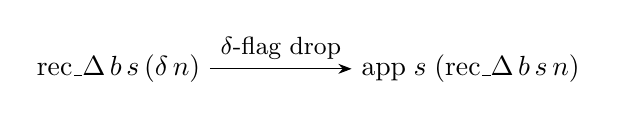
\begin{tikzpicture}[node distance=18mm, >=Stealth]
  \node (t0) {$\mathrm{rec}\_\Delta\,b\,s\,(\delta\,n)$};
  \node (t1) [right=of t0] {$\mathrm{app}\;s\;(\mathrm{rec}\_\Delta\,b\,s\,n)$};
  \draw[->] (t0) -- (t1) node[midway, above] {\small $\delta$-flag drop};
\end{tikzpicture}
\end{center}

\section{Impossibility results}
\label{sec:impossibility}
We formally establish the failure of several simpler measure strategies, which necessitate the use of DM multiset orders or MPO. These negative results are verified in the formal development.

\begin{itemize}[leftmargin=1.4em]
  \item \textbf{Additive bumps fail}: No measure of the form $\kappa(t) + k$ strictly decreases on generic duplicating rules.
  \item \textbf{Bare flags fail}: A single boolean flag is insufficient to orient rules that lift depth.
  \item \textbf{Polynomial interpretations fail}: Any polynomial interpretation involving fixed constants requires external arithmetic axioms to ``orient'' the rule, violating the operator-only constraint.
\end{itemize}

\paragraph{Polynomial Impossibility.}
Consider polynomial interpretations of the form $M(t) \in \mathbb{N}$ for a duplicating rule $f(x) \to g(x, x)$. A polynomial measure assigning $M(f(x)) = M(x) + p$ requires $M(x) + p > 2M(x)$ for strict decrease, implying $p > M(x)$. This fails for unbounded $M(x)$.

More generally: any polynomial proof for a system with duplicating rules must hardcode specific constants (e.g., $M(\mathrm{void})=2$) to satisfy inequalities like $2M(s) > M(s) + 1$. Such proofs import external arithmetic properties and impose arbitrary values on operators, violating the principle that operators' semantics should be defined solely by rewrite rules. Changing the hardcoded constant (e.g., $M(\mathrm{void})=1$) collapses the proof. This structural failure is why polynomial interpretations cannot orient generic duplicating rules without external axioms.

\paragraph{Internally definable measures.}
We use a simple contract for internally defined termination measures to structure these negative results:
\begin{definition}[Internally definable measure]
An internally definable measure for a type $\alpha$ consists of $(\beta,\;<\_{\beta},\;\mathsf{wf},\;m,\;\mathsf{ctxMono},\;\mathsf{piecesLt})$ where: $\beta$ is a base order carrier; $<\_{\beta}$ is a well-founded relation with witness $\mathsf{wf}$; $m: \alpha\to\beta$ is the measure; $\mathsf{ctxMono}$ expresses context compatibility; and $\mathsf{piecesLt}$ asserts that in each rule instance, every RHS piece is strictly smaller than the removed LHS redex w.r.t. $<\_{\beta}$.
\end{definition}

\section{Decidability of Reachability}
\label{sec:decidability}
\begin{theorem}[Fixed-target reachability]
In a strongly normalizing TRS, the set $\{t \mid t \Rightarrow^* c\}$ for any constant $c$ is decidable via normalization.
\end{theorem}

This connects our work to classical results: if we could encode undecidable properties through reduction to constants, we would violate known theoretical limits. This motivates stratified approaches in proof assistants, where object-level and meta-level reasoning are carefully separated.

\paragraph{Assumptions (model).} We work with a finite first-order TRS over finite terms. The decision method is: compute a normal form (by SN) and check whether it is $\top$; with local confluence, this reduces to one normalization and an equality test.

\paragraph{Complexity context.} Small-term reachability in terminating TRSs ranges from NP (length-reducing) to NExpTime/N2ExpTime (polynomial interpretations) and PSPACE (KBO), with confluence lowering the length-reducing class to P \cite{BaaderGiesl24}. This situates our ``normalize and compare'' decision procedure for KO7 within the established landscape.

Moreover, decidability can be \emph{modular} for disjoint unions under left-linearity/non-collapsing assumptions \cite{CaronCoquide94}, while termination alone does not guarantee decidability: even \emph{flat} non-linear TRSs have undecidable reachability/joinability/confluence \cite{Mitsuhashi06}.

\section{Conjecture: Full Termination of Any Relational Operator-Only TRS}
\label{sec:conjecture}

\paragraph{What ``relational'' means.}
A \emph{relational} operator-only TRS is, by definition, one capable of \emph{ordered computation}. The terms are equivalent: ``relational'' = ``capable of ordered computation.'' Such systems can express iteration over successors, comparison of structure depths, or any form of sequential counting. The minimal signature for such capability includes a recursor, an operator that applies a step function iteratively across a successor-structured argument. Examples include primitive recursion over natural numbers, fold over lists, and any construct that steps through an ordered index. A TRS that cannot express such iteration (e.g., a flat pattern-matching system with no recursive structure) is not relational in this sense.

The critical property of relational systems is that their recursor \emph{redistributes} its step argument across recursive calls. This redistribution is not optional: it is what makes ordered computation possible. But it also defeats all additive termination measures.

\paragraph{The structural barrier.}
Any operator system capable of ordered computation requires a recursor. A recursor redistributes its step argument across recursive calls. This redistribution defeats additive termination measures: $M(\text{after}) = M(\text{before}) - 1 + M(s)$, yielding no strict drop when $M(s) \ge 1$.

\begin{definition}[Internally definable measure]\label{def:internal}
An internally definable termination method for signature $\Sigma$ uses only: simplification orders with fixed precedence/status on $\Sigma$ (LPO/RPO/MPO), DM-multiset lifts of $\mathbb{N}$-valued ranks, and algebraic interpretations definable without importing external axioms. No encodings into external arithmetic, no borrowed logic, and no hard-coded constants outside the operator language.
\end{definition}

\begin{conjecture}[Full Termination Conjecture for Relational TRSs]\label{conj:main}
No relational operator-only TRS can have its full-system termination proved by internally definable methods. Specifically: let $R$ be an operator-only TRS with a recursor rule of the form
\[
\mathrm{rec}(b, s, \sigma(n)) \to f(s, \mathrm{rec}(b, s, n)).
\]
No internally definable measure (Definition~\ref{def:internal}) proves termination of $R$ when the step argument $s$ is unrestricted. The structural redistribution of $s$ into both the function application and the recursive call defeats every additive, polynomial, or path-order measure that does not import external arithmetic or ordinal axioms. Any proof that relies on external axioms, imported arithmetic, or meta-level encodings is outside scope and does not count as an internal termination argument.
\end{conjecture}

\paragraph{Scope of the conjecture.}
The conjecture applies to any TRS expressive enough to encode ordered data (natural numbers, lists, trees with successor structure, or any type supporting iteration). Systems without such structure (purely ground, non-recursive, or lacking a step-iteration pattern) fall outside the conjecture's scope. The claim is that \emph{once a system has enough structure for ordered computation, its full termination escapes internal proof methods}.

\paragraph{Evidence.} In KO7, the \texttt{rec-succ} rule has the critical shape: the step argument $s$ appears twice on the RHS, and when $s$ contains nested redexes, every additive measure fails to decrease strictly. The redistribution identity $M(\text{after}) = M(\text{before}) - 1 + M(s)$ yields no strict drop when $M(s) \ge 1$. The guarded SafeStep fragment terminates because the $\delta$-phase bit restricts allowable step arguments; without such restriction, the full system admits unbounded recursive depth. The gap between internally definable ranking functions and what would be required cannot be closed without external methods (axioms, encodings, or borrowed arithmetic).

\section{Formalization structure}
\label{sec:formalization}
The formal verification is implemented in a proof assistant. The project structure separates the kernel definitions, meta-theory proofs, and impossibility results:
\begin{itemize}[leftmargin=1.3em]
  \item \textbf{Termination proofs:} Establishes the per-rule decreases and strong normalization for the safe fragment using the triple-lexicographic measure.
  \item \textbf{Normalization:} Defines the normalization function and proves its totality and soundness.
  \item \textbf{Confluence:} Implements the Newman engine and the star-star join, relying on local join lemmas.
  \item \textbf{Impossibility results:} Contains the verified counterexamples for additive measures and the proofs that simple measures fail under duplication.
\end{itemize}
All claimed results are formally proven without reliance on unproven postulates in the current build. The formal development is available at \url{https://github.com/MosesRahnama/OperatorKO7}.

\section*{Acknowledgments}
AI has been a great help with this project.

\section*{References}
\addcontentsline{toc}{section}{References}
\begingroup
\small
\renewcommand{\refname}{}
\bibliographystyle{plain}
\bibliography{references}
\endgroup

\appendix
\section*{Appendix: Addendum}

\subsection*{KO7 Rules Table (7 constructors, 8 rules)}
\begin{table}[h]
  \centering
  \begin{tabular}{@{}llcll@{}}
    \toprule
    Rule & Head & Arity & Shape & Dup? \\
    \midrule
    \texttt{R\_merge\_void\_left} & merge & 2 & $\mathrm{merge}\;\mathrm{void}\;t \to t$ & No \\
    \texttt{R\_merge\_void\_right} & merge & 2 & $\mathrm{merge}\;t\;\mathrm{void} \to t$ & No \\
    \texttt{R\_merge\_cancel} & merge & 2 & $\mathrm{merge}\;t\;t \to t$ & No \\
    \texttt{R\_rec\_zero} & rec$\Delta$ & 3 & $\mathrm{rec}\,\Delta\,b\,s\,\mathrm{void} \to b$ & No \\
    \texttt{R\_rec\_succ} & rec$\Delta$ & 3 & $\mathrm{rec}\,\Delta\,b\,s\,(\mathrm{delta}\,n) \to \mathrm{app}\,s\,(\mathrm{rec}\,\Delta\,b\,s\,n)$ & No$^*$ \\
    \texttt{R\_int\_delta} & integrate & 1 & $\mathrm{integrate}\,(\mathrm{delta}\,t) \to \mathrm{void}$ & No \\
    \texttt{R\_eq\_refl} & eqW & 2 & $\mathrm{eqW}\;a\;a \to \mathrm{void}$ & No \\
    \texttt{R\_eq\_diff} & eqW & 2 & $\mathrm{eqW}\;a\;b \to \mathrm{integrate}\,(\mathrm{merge}\,a\,b)$ & No \\
    \bottomrule
  \end{tabular}
  \caption{KO7's 8 kernel rules (appendix copy). In the full kernel relation, \texttt{R\_eq\_refl} and \texttt{R\_eq\_diff} overlap at \texttt{eqW a a}. The certified safe fragment guards \texttt{R\_eq\_diff} by $a \neq b$. \texttt{R\_merge\_cancel} is collapsing (erases one copy). $^*$\texttt{R\_rec\_succ} redistributes $s$ to two positions on the RHS; see Remark below.}
\end{table}

\subsection*{Lean kernel location}
The authoritative mechanized kernel is the Lean file \texttt{OperatorKO7/Kernel.lean} in the repository \url{https://github.com/MosesRahnama/OperatorKO7}. The safe fragment and proofs are under \texttt{OperatorKO7/Meta/}.

\subsection*{Triple-lexicographic measure and duplication handling (DM/MPO)}
We order $\mu^3(t) = (\delta\text{-flag}(t),\, \kappa^{M}(t),\, \mu_{\mathrm{ord}}(t))$ by lex:
\begin{itemize}[leftmargin=1.4em]
  \item $\delta$-flag: phase bit dropping on the successor recursion branch.
  \item Multiset $\kappa^{M}$: a Dershowitz-Manna multiset extension over a base precedence/status (or MPO head precedence) orienting redexes strictly above pieces; covers duplicators.
  \item Ordinal $\mu_{\mathrm{ord}}$: resolves non-duplicating ties; right-addition is not strictly monotone; absorption $\alpha + \beta = \beta$ needs $\omega \le \beta$.
\end{itemize}
Per-rule lemmas show every RHS component is strictly smaller than the removed redex in the base order.

\paragraph{Aggregation for $\kappa^{M}$ (union, not sum).}
We emphasize that $\kappa^{M}$ aggregates via \emph{multiset union} ($\cup$), not numeric addition. For duplicating rules, the multiset of piece-weights on the RHS is DM-smaller than the singleton multiset containing the LHS redex weight, yielding a strict drop in the $\kappa^{M}$ component. For non-duplicating rules, $\kappa^{M}$ ties by definitional equality and the ordinal $\mu_{\mathrm{ord}}$ resolves the branch. In particular, for unguarded instances of \texttt{eqW}-refl and merge-cancel we use a $\kappa$-branch: when $\kappa^{M}(a) \ne 0$ we obtain a left-lex drop via DM; when $\kappa^{M}(a)=0$ the $\kappa^{M}$ component ties by \texttt{rfl} and the strict decrease is witnessed in the $\mu_{\mathrm{ord}}$ coordinate (right branch of \texttt{Prod.Lex}).

\paragraph{Short witness snippets (toy duplication).}
Toy rule: $\mathrm{pair}(\mathrm{s}\,x,\,y) \to \mathrm{pair}(x,\,\mathrm{pair}(y,\,y))$.

\emph{DM multiset on sizes.} Let $S(x,y)=\mathrm{size}(\mathrm{pair}(\mathrm{s}\,x,\,y))=\mathrm{size}(x)+\mathrm{size}(y)+2$. Then $\mathrm{size}(x) < S(x,y)$ and $\mathrm{size}(y) < S(x,y)$. Use $X=\varnothing$, $Y=\{\mathrm{size}(x),\mathrm{size}(y)\}$, $Z=\{S(x,y)\}$ to conclude $Y <_{\mathrm{DM}} Z$.

\emph{MPO triple weight.} $\mathrm{weight}(\mathrm{pair}\,a\,b)=(\mathrm{headRank}(a),\,\mathrm{size}(a),\,\mathrm{size}(b))$ with $\mathrm{headRank}(\mathrm{s}\,\_) = 2$, else $1$. If $x$ is unit/pair then first components decrease (1<2). If $x=\mathrm{s}\,t$ then tie on 2; the second components satisfy $\mathrm{size}(t)+1<\mathrm{size}(t)+2$.

\begin{figure}[h]
  \centering
  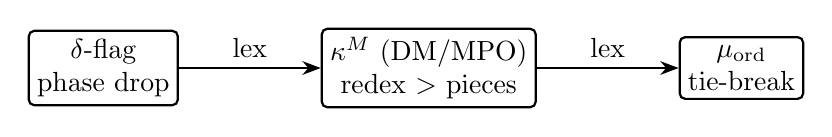
\begin{tikzpicture}[node distance=12mm, >=Stealth, thick]
    \node[draw, rounded corners=2pt, inner sep=3pt, align=center] (delta) {$\delta$-flag\\phase drop};
    \node[draw, rounded corners=2pt, inner sep=3pt, align=center, right=18mm of delta] (kappa) {$\kappa^{M}$ (DM/MPO)\\redex $>$ pieces};
    \node[draw, rounded corners=2pt, inner sep=3pt, align=center, right=18mm of kappa] (mu) {$\mu_{\mathrm{ord}}$\\tie-break};
    \draw[->] (delta) -- node[above]{lex} (kappa);
    \draw[->] (kappa) -- node[above]{lex} (mu);
  \end{tikzpicture}
  \caption{Triple-lex measure components. Duplicators decrease via $\kappa^{M}$; non-duplicating ties via $\mu_{\mathrm{ord}}$.}
\end{figure}

\subsection*{Newman scope (guarded safe relation)}
SN + local confluence implies confluence; in the artifact this is instantiated for the \emph{safe} relation via an Acc-based star-star join. Scope note: all confluence statements and their Newman instantiations are for \emph{SafeStep} only. Full Step is \emph{not} locally joinable at root for \texttt{eqW}\,a\,a with $\kappa^{M}(a)=0$; accordingly we do not claim full-step confluence.

\subsection*{Module map}
The verification logic is distributed across key modules for SN, normalizer, and confluence engine. Local confluence lemmas are proved separately. Note: context closure and local-join lemmas are explicitly instantiated for the \emph{SafeStep} fragment (\texttt{SafeStepCtx}) rather than the full relation.

\subsection*{Per-rule orientation (DM/MPO/$\delta$/$\mu$)}
\begin{table}[h]
  \centering
  \scriptsize
  \setlength{\tabcolsep}{4pt}
  \begin{tabularx}{\textwidth}{@{}l l Y Y l@{}}
    Rule & Base component & Precedence/Status & Witness & Source \\
    \midrule
    merge void left & $\mu$ (ordinal) & (n/a) & Theorem 4.1 & Termination \\
    merge void right & $\mu$ (ordinal) & (n/a) & Theorem 4.2 & Termination \\
    merge cancel & DM on $\kappa^M$ (redex $>$ pieces) & head precedence & Theorem 4.3 & Termination \\
    rec zero & DM on $\kappa^M$ & rec $>$ pieces & Theorem 4.4 & Termination \\
    rec succ & $\delta$ phase bit (1 $\to$ 0) & (n/a) & Theorem 4.5 & Termination \\
    eqW refl & MPO ($\mu$-first triple) & head precedence & Theorem 4.6 & Termination \\
    eqW diff & MPO ($\mu$-first triple) & head precedence & Theorem 4.7 & Termination \\
    integrate (delta t) & $\mu$ (unique target) & (n/a) & Theorem 4.8 & Termination \\
    toy duplication & DM on size & s $>$ pair & Lemma 7.1 & Impossibility \\
    toy duplication & MPO triple & headRank(s) $>$ headRank(pair) & Lemma 7.2 & Impossibility \\
    \bottomrule
  \end{tabularx}
  \caption{Per-rule orientation summary.}
\end{table}

Parenthetical aliases: for substitution convenience we expose simp forms alongside the main rec lemmas.

\subsection*{Local-join report (critical peaks and unique-target cases)}
\begin{table}[h]
  \centering
  \footnotesize
  \setlength{\tabcolsep}{4pt}
  \begin{tabularx}{\textwidth}{@{}l l Y@{}}
    Shape & Join lemma name & Notes \\
    \midrule
    merge void void & \texttt{localJoin\_merge\_void\_void} & both branches to void \\
    merge t t & \texttt{localJoin\_merge\_tt} & joins at $t$ (context-lifted) \\
    integrate (delta t) & \texttt{localJoin\_int\_delta} & unique target void \\
    rec$\Delta$ b s void & \texttt{localJoin\_rec\_zero} & unique target b \\
    rec$\Delta$ b s (delta n) & \texttt{localJoin\_rec\_succ} & unique target app s (rec$\Delta$ b s n) \\
    eqW a b, a $\ne$ b & \texttt{localJoin\_eqW\_ne} & only diff applies (unique target) \\
    eqW a a, guard kappaM a $\ne$ 0 & \texttt{localJoin\_eqW\_refl\_guard\_ne} & refl blocked; only diff \\
    merge a b (no void, a $\ne$ b) & \texttt{localJoin\_merge\_no\_void\_neq} & no root step; vacuous \\
    integrate non-delta & \texttt{localJoin\_integrate\_non\_delta} & no root step; vacuous \\
    rec$\Delta$ b s n (n $\ne$ void, not delta) & \texttt{localJoin\_rec\_other} & no root step; vacuous \\
    \bottomrule
  \end{tabularx}
  \caption{Local-join witnesses for the safe relation (root).}
\end{table}

\subsection*{Ctx-local join wrappers}
When needed in context, the root local-join lemmas lift to context via wrappers:
\begin{table}[h]
  \centering
  \footnotesize
  \setlength{\tabcolsep}{4pt}
  \begin{tabularx}{\textwidth}{@{}l l Y@{}}
    Shape & Ctx wrapper lemma & Notes \\
    \midrule
    merge a b (no void, a $\ne$ b) & \texttt{localJoin\_ctx\_merge\_no\_void\_neq} & from root `merge' lemma \\
    eqW a b, a $\ne$ b & \texttt{localJoin\_ctx\_eqW\_ne} & only diff applies \\
    eqW a a, kappaM guard & \texttt{localJoin\_ctx\_eqW\_refl\_guard\_ne} & refl blocked \\
    eqW a a if merge$\to$delta & \texttt{localJoin\_ctx\_eqW\_refl\_if\_merge\_normalizes\_to\_delta} & via normalizeSafe \\
    eqW a a if integrate$\to$void & \texttt{localJoin\_ctx\_eqW\_refl\_if\_integrate\_merge\_to\_void} & via ctx star \\
    eqW (delta n) (delta n) & \texttt{localJoin\_ctx\_eqW\_refl\_when\_a\_is\_delta} & literal delta case \\
    \bottomrule
  \end{tabularx}
  \caption{Ctx-local join wrappers.}
\end{table}

\section*{Appendix: Orientation Strategy}
This summarizes the exact orientation strategy realized in the proofs (no global RPO required):
\begin{itemize}[leftmargin=1.3em]
  \item Non-duplicating rules use a \emph{$\mu$-first} lex measure: triples $(\mu, \mathrm{sizeMPO}, \delta)$ decrease directly via lemmas.
  \item The rule \texttt{rec\_zero} uses a \emph{DM multiset} drop on $\kappa^M$, wrapped by \texttt{drop\_R\_rec\_zero}.
  \item The rule \texttt{rec\_succ} drops the \emph{$\delta$ phase bit} (1\,$\to$\,0) via \texttt{drop\_R\_rec\_succ}.
  \item Merge-cancel decreases via DM on $\kappa^M$ under a base precedence where the redex strictly dominates its pieces.
  \item Conceptual precedence (if one prefers an MPO reading) aligns with rec $>$ merge $>$ app $>$ integrate $>$ eqW $>$ delta $>$ void, but the formal proofs do not require a global precedence declaration.
\end{itemize}
Formal anchors:
\begin{itemize}[leftmargin=1.3em]
  \item Merge void left/right: $\mu$-first or DM tie plus $\mu$.
  \item Merge cancel: DM multiset drop on $\kappa^M$.
  \item Rec zero: \texttt{drop\_R\_rec\_zero} with \texttt{dm\_drop\_R\_rec\_zero} for the inner DM piece.
  \item Rec succ: \texttt{drop\_R\_rec\_succ} via the $\delta$ phase bit (1 $\to$ 0).
  \item EqW refl/diff: $\mu$-first MPO triple.
  \item Integrate delta: unique target \texttt{void}.
\end{itemize}

\section{Related work}
\label{sec:related}
We follow standard expositions in Baader-Nipkow and Terese \cite{BaaderNipkow98,Terese03}. Termination under duplication relies on DM multiset orders \cite{DershowitzManna79} and (recursive) path orders \cite{Dershowitz87}. Newman's Lemma is used in its classic ARS form \cite{Newman42}. For independence via termination, see Goodstein and Kirby-Paris and ordinal tools due to Buchholz \cite{Goodstein44,KirbyParis82,Buchholz86}. For fixed-target reachability complexity and modularity results, see \cite{BaaderGiesl24,CaronCoquide94}; for undecidability at shallow depth in non-linear systems, see \cite{Mitsuhashi06}.

\section{Conclusion}
We gave an operator-only kernel and proved \emph{strong normalization and confluence for the guarded safe subrelation}, yielding a certified normalizer and unique normal forms via Newman's Lemma. We also established an explicit non-local-join witness at the eqW reflexive peak (under $\kappa^M=0$), blocking confluence for the \emph{full} relation; this motivates the designed SafeStep fragment. A decidability result explains why single-level G\"odel encodings clash with global termination. We proved a simple impossibility for additive bumps under duplication and certified DM/MPO orientations. Future work: complete a stratified meta-layer; develop arithmetic encodings within KO7; and map the exact boundary between internally definable measures and external ordinal strength.

\end{document}

